%\documentclass[11pt]{article}

\documentclass[addpoints,10pt]{exam}

\usepackage[margin=2.5cm]{geometry}
\usepackage{graphicx}
\usepackage{listings}
\usepackage{xpatch}
\usepackage{color}
\usepackage{amsmath}
\usepackage[spanish]{babel}

\makeatletter
\xpretocmd{\item@points@pageinfo}{\normalfont}{}{}
\xapptocmd{\item@points@pageinfo}{\bfseries}{}{}
\makeatother

\begin{document}
	\begin{center}
		\LARGE\scshape{Microscopio optico}
		
		\vspace{1cm}
		\large\scshape{Juan Barbosa - 201325901}
	\end{center}

	En el centro de microscop\'ia el d\'ia martes realizamos la pr\'actica de alineaci\'on del microscopio con iluminaci\'on K\"ohler. Adicional a esto observamos en detalle dos elementos que componen la parte \'optica del microscopio. Los elementos observados fueron:
	
	\paragraph{Diafragma}
	permite regular la cantidad de luz que pasa sobre ciertas partes del microscopio. En el caso del microscopio usado existen dos diafragmas, siguiendo el camino \'optico, el primero es el de campo y el segundo el del condensador. La regulaci\'on de la cantidad de luz se da al limitar la apertura del diafragma.
	\begin{figure}[h]
		\centering
		\begin{tabular}{cc}
			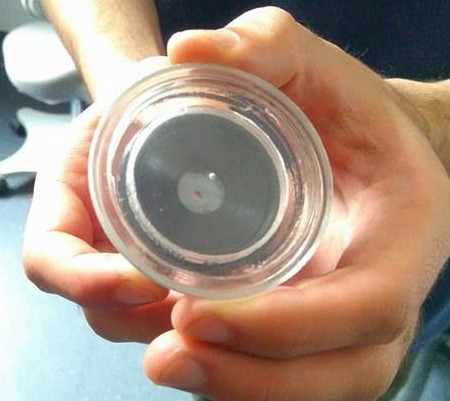
\includegraphics[width = 0.3\linewidth]{diafragma1.jpg} & 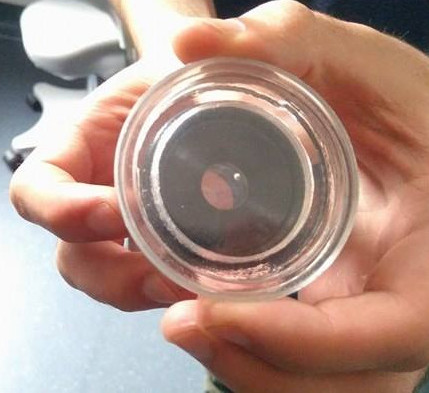
\includegraphics[width = 0.3\linewidth]{diafragma2.jpg}\\
		\end{tabular}
		\caption{Diafragma cerrado y diafragma abierto.}
	\end{figure}
	
	\paragraph{Objetivo}
	El objetivo constituye el elemento \'optico m\'as cercano a la muestra. La magnificaci\'on del objetivo es la de mayor contribuci\'on a la magnificaci\'on total de la muestra. La mayor\'ia de objetivos tienen rangos de 10x a 100x. Los objetivos presentan diversas caracter\'isticas entre las cuales se destaca el m\'edio en el que funcionan.
	\begin{figure}[h]
		\centering
		\begin{tabular}{cc}
			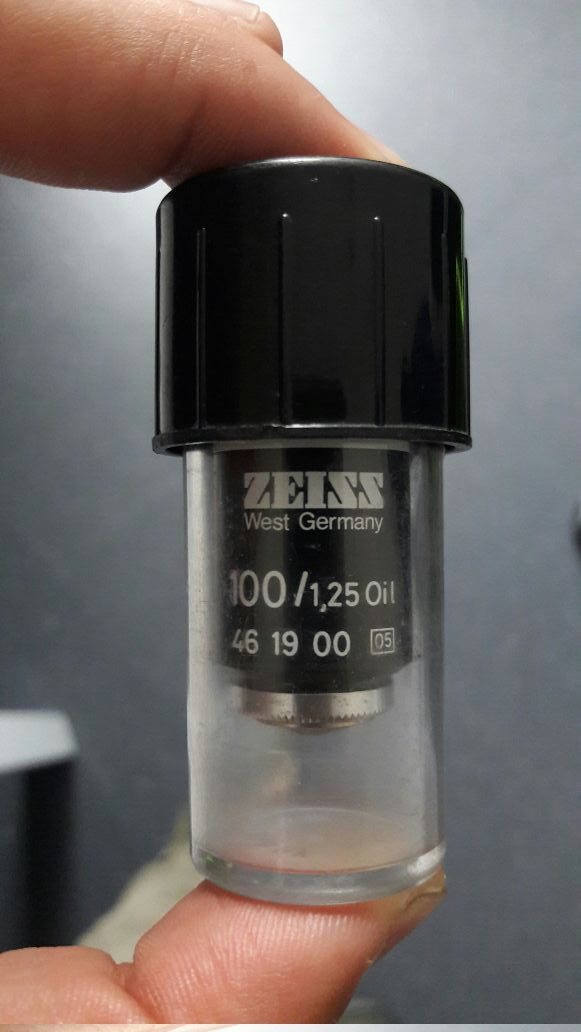
\includegraphics[width = 0.2\linewidth]{objetivo.jpg} &
			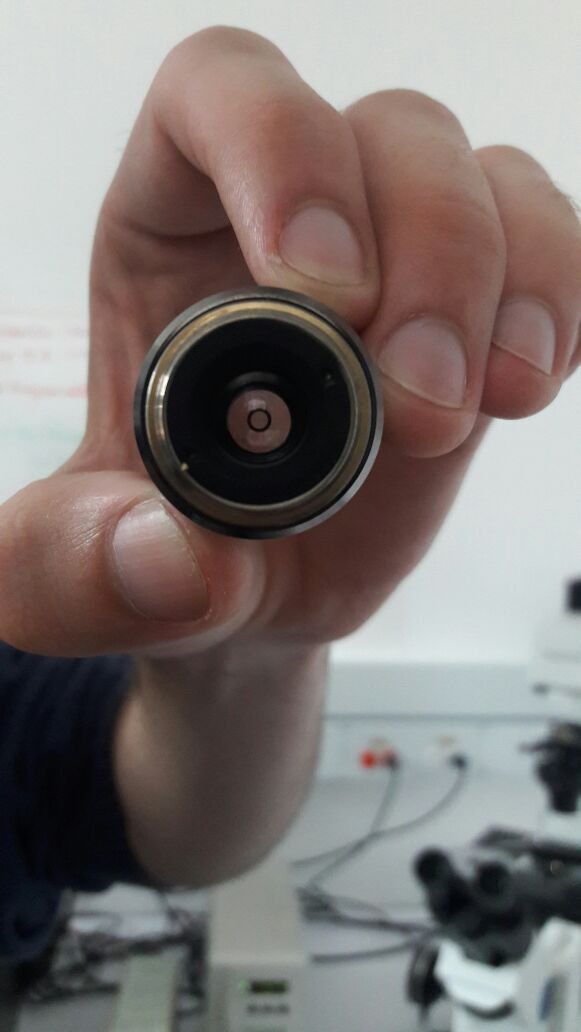
\includegraphics[width = 0.2\linewidth]{DIC.jpg}
		\end{tabular}
		
		\caption{Ejemplos de objetivos. Para la imagen izquierda, la magnificaci\'on es de 100x, se debe usar aceite de inmersi\'on, y la apertura num\'erica es de 1.25. A la derecha imagen del anillo de un objetivo para DIC.}
	\end{figure}
	
	\newpage
	Sobre el microsc\'opio se estudi\'o el efecto del diafragma del condensador. El cual enfoca la luz sobre la muestra.
	\begin{figure}[h]
		\centering
		\begin{tabular}{cc}
			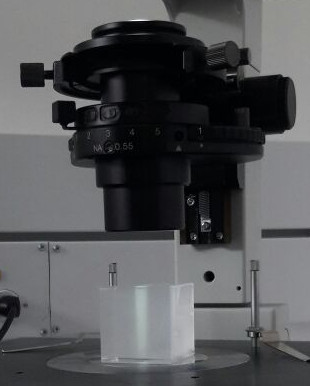
\includegraphics[width = 0.3\linewidth]{condensador1.jpg} &
			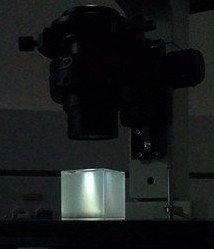
\includegraphics[width = 0.3\linewidth]{condensador2.jpg}
		\end{tabular}
		\caption{Efecto del diafragma del condensador. El control de la apertura determina el \'angulo del cono de luz. En general se quiere que el cono se enfoque sobre la muestra (izquierdo).}
	\end{figure}
	
	Luego analizar los elementos antes mencionados tuvo lugar la alineaci\'on del microscopio con iluminaci\'on K\"ohler, para lo cual se abrieron completamente ambos diafragmas y se enfoc\'o la muestra. Posteriormente se baj\'o completamente el condensador y se cerr\'o el diafragma de campo. Se busca la imagen del diafragma en el campo de visi\'on. En este punto el diafragma se observa circular, subiendo gradualmente el condensador se observa el oct\'agono del diafragma. Posteriormente se centra la imagen del mismo y se abre hasta no ver el borde.
	\begin{figure}[h]
		\centering
		\begin{tabular}{cc}
			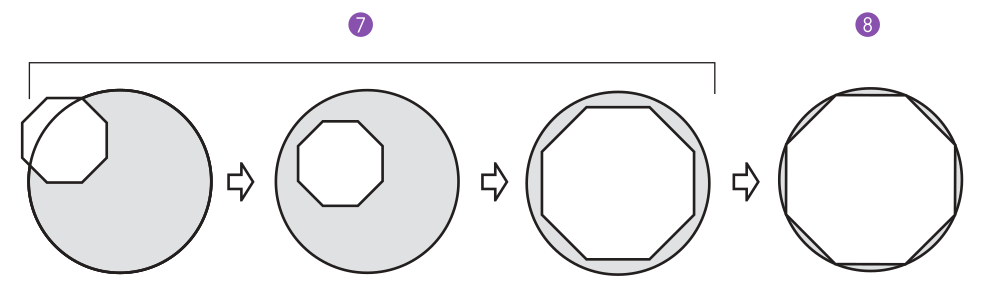
\includegraphics[width=0.5\linewidth]{alineacion.png} & 
			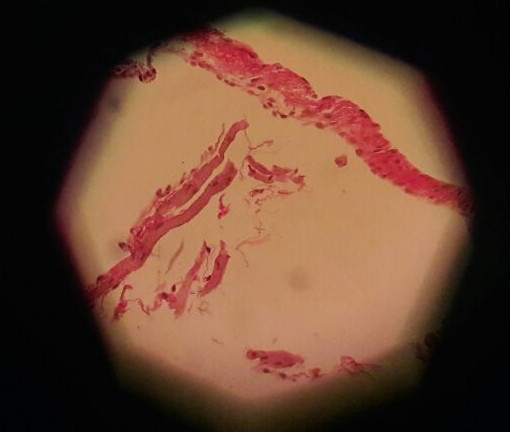
\includegraphics[width=0.2\linewidth]{alineacion.jpg}
		\end{tabular}
		\caption{A la izquierda, alineaci\'on del diafragma del condensador \cite{Olympus}. A la derecha, observado en el laboratorio.}
	\end{figure}
	
	Finalmente se removi\'o el ocular y se observ\'o la proyecci\'on de la muestra en el techo. Adem\'as se dispuso del telesc\'opio de centrado para observar la bombilla de iluminaci\'on \cite{Olympus}.
	
	\begin{figure}[h]
		\centering
		\begin{tabular}{cc}
			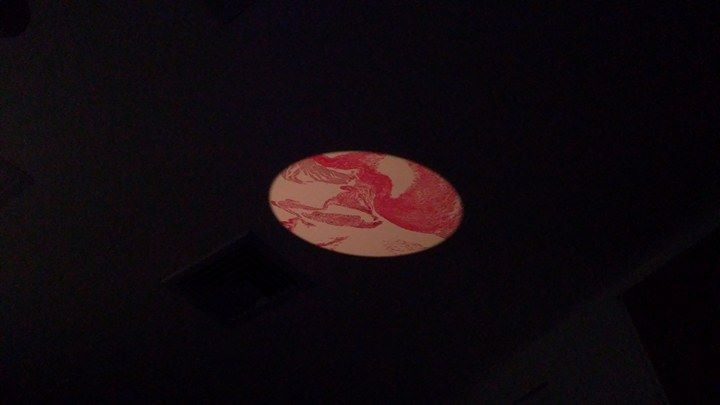
\includegraphics[width = 0.4\linewidth]{proyeccion.jpg} & 
			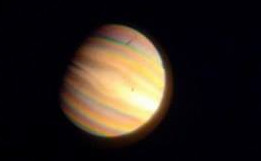
\includegraphics[width = 0.35\linewidth]{bombilla.jpg}
		\end{tabular}
		\caption{A la izquierda, proyecci\'on de la muestra. A la derecha, bombilla de iluminaci\'on.}
	\end{figure}


	\begin{thebibliography}{9}
		\bibitem{Olympus} 
		Basics of Inverted Microscope, Olympus. 2012 
	\end{thebibliography}	
\end{document}
